\documentclass{article}

\usepackage[utf8]{inputenc}
\usepackage{hyperref}
\usepackage{listings}
\usepackage{graphicx}
\usepackage{listings}

\title{Lab Sheet 3}
\date{Security}

\begin{document}
\maketitle

In our third lab, we will use \href{https://www.cyberpunk.rs/password-cracker-thc-hydra}{hydra}, a tool in Kali Linux, to perform a Brute Force attack on a Web based login. Hydra is the fastest network logon cracker which supports numerous attack protocols. It is very fast and flexible, and new modules are easy to add. This tool makes it possible for researchers and security consultants to show how easy it would be to gain unauthorized access to a system remotely. 

\section{Task 1: Brute Force Web-based Login with hydra}
We will use http to run a brute force attack on a vulnerability testing site.

\subsection{Get to know your tool}
Type \texttt{hydra -h} (\texttt{h} for help) in your Kali terminal and find out what \textit{hydra} is all about and how it might work.

\subsection{}
One of hydra's brute force attackingservices is used on Web-based logins, such as social media login forms, user banking login forms, your router's Web-based login, etc. That's \texttt{http[s]-{get|post}-form} which will handle this request.

Before we fire up hydra, we should know some of the arguments:
\begin{itemize}
\item \textbf{Target:} http://testasp.vulnweb.com/Login.asp?RetURL=\%2FDefault\%2Easp\%3F
\item \textbf{Login username:} admin (if you're not sure, bruteforce this)
\item \textbf{Password list:} ``The location of the dictionary file list containing possible passwords.''
\item \textbf{Form parameters:} ``Here we will be using iceweasel or firefox network developer toolbar.''
\item \textbf{Service module:} http-post-form
\end{itemize}

\subsection{Obtaining post parametres}
Visit \href{http://testasp.vulnweb.com/Login.asp?RetURL=\%2FDefault\%2Easp\%3F}{http://testasp.vulnweb.com/Login.asp?RetURL=\%2FDefault\%2Easp\%3F} and open the \textit{Network} tool in the \textit{Web Developer} menu.

To obtain the post-form parameters, type anything in the \textit{username} and/or \textit{password} form. You will notice a new \textbf{POST} method on the network developer tab. Click on that line and on the \textit{Headers} tab click \textit{Edit and Resend} on the right side. From the \textit{Request Body} textbox, copy the last line, e.g. \texttt{tfUName=admin\&tfUPass=password}. The \textit{tfUName} and \textit{tfUPass} are parameters we need (see Figure 1).

\begin{figure}[h]
  \centering
  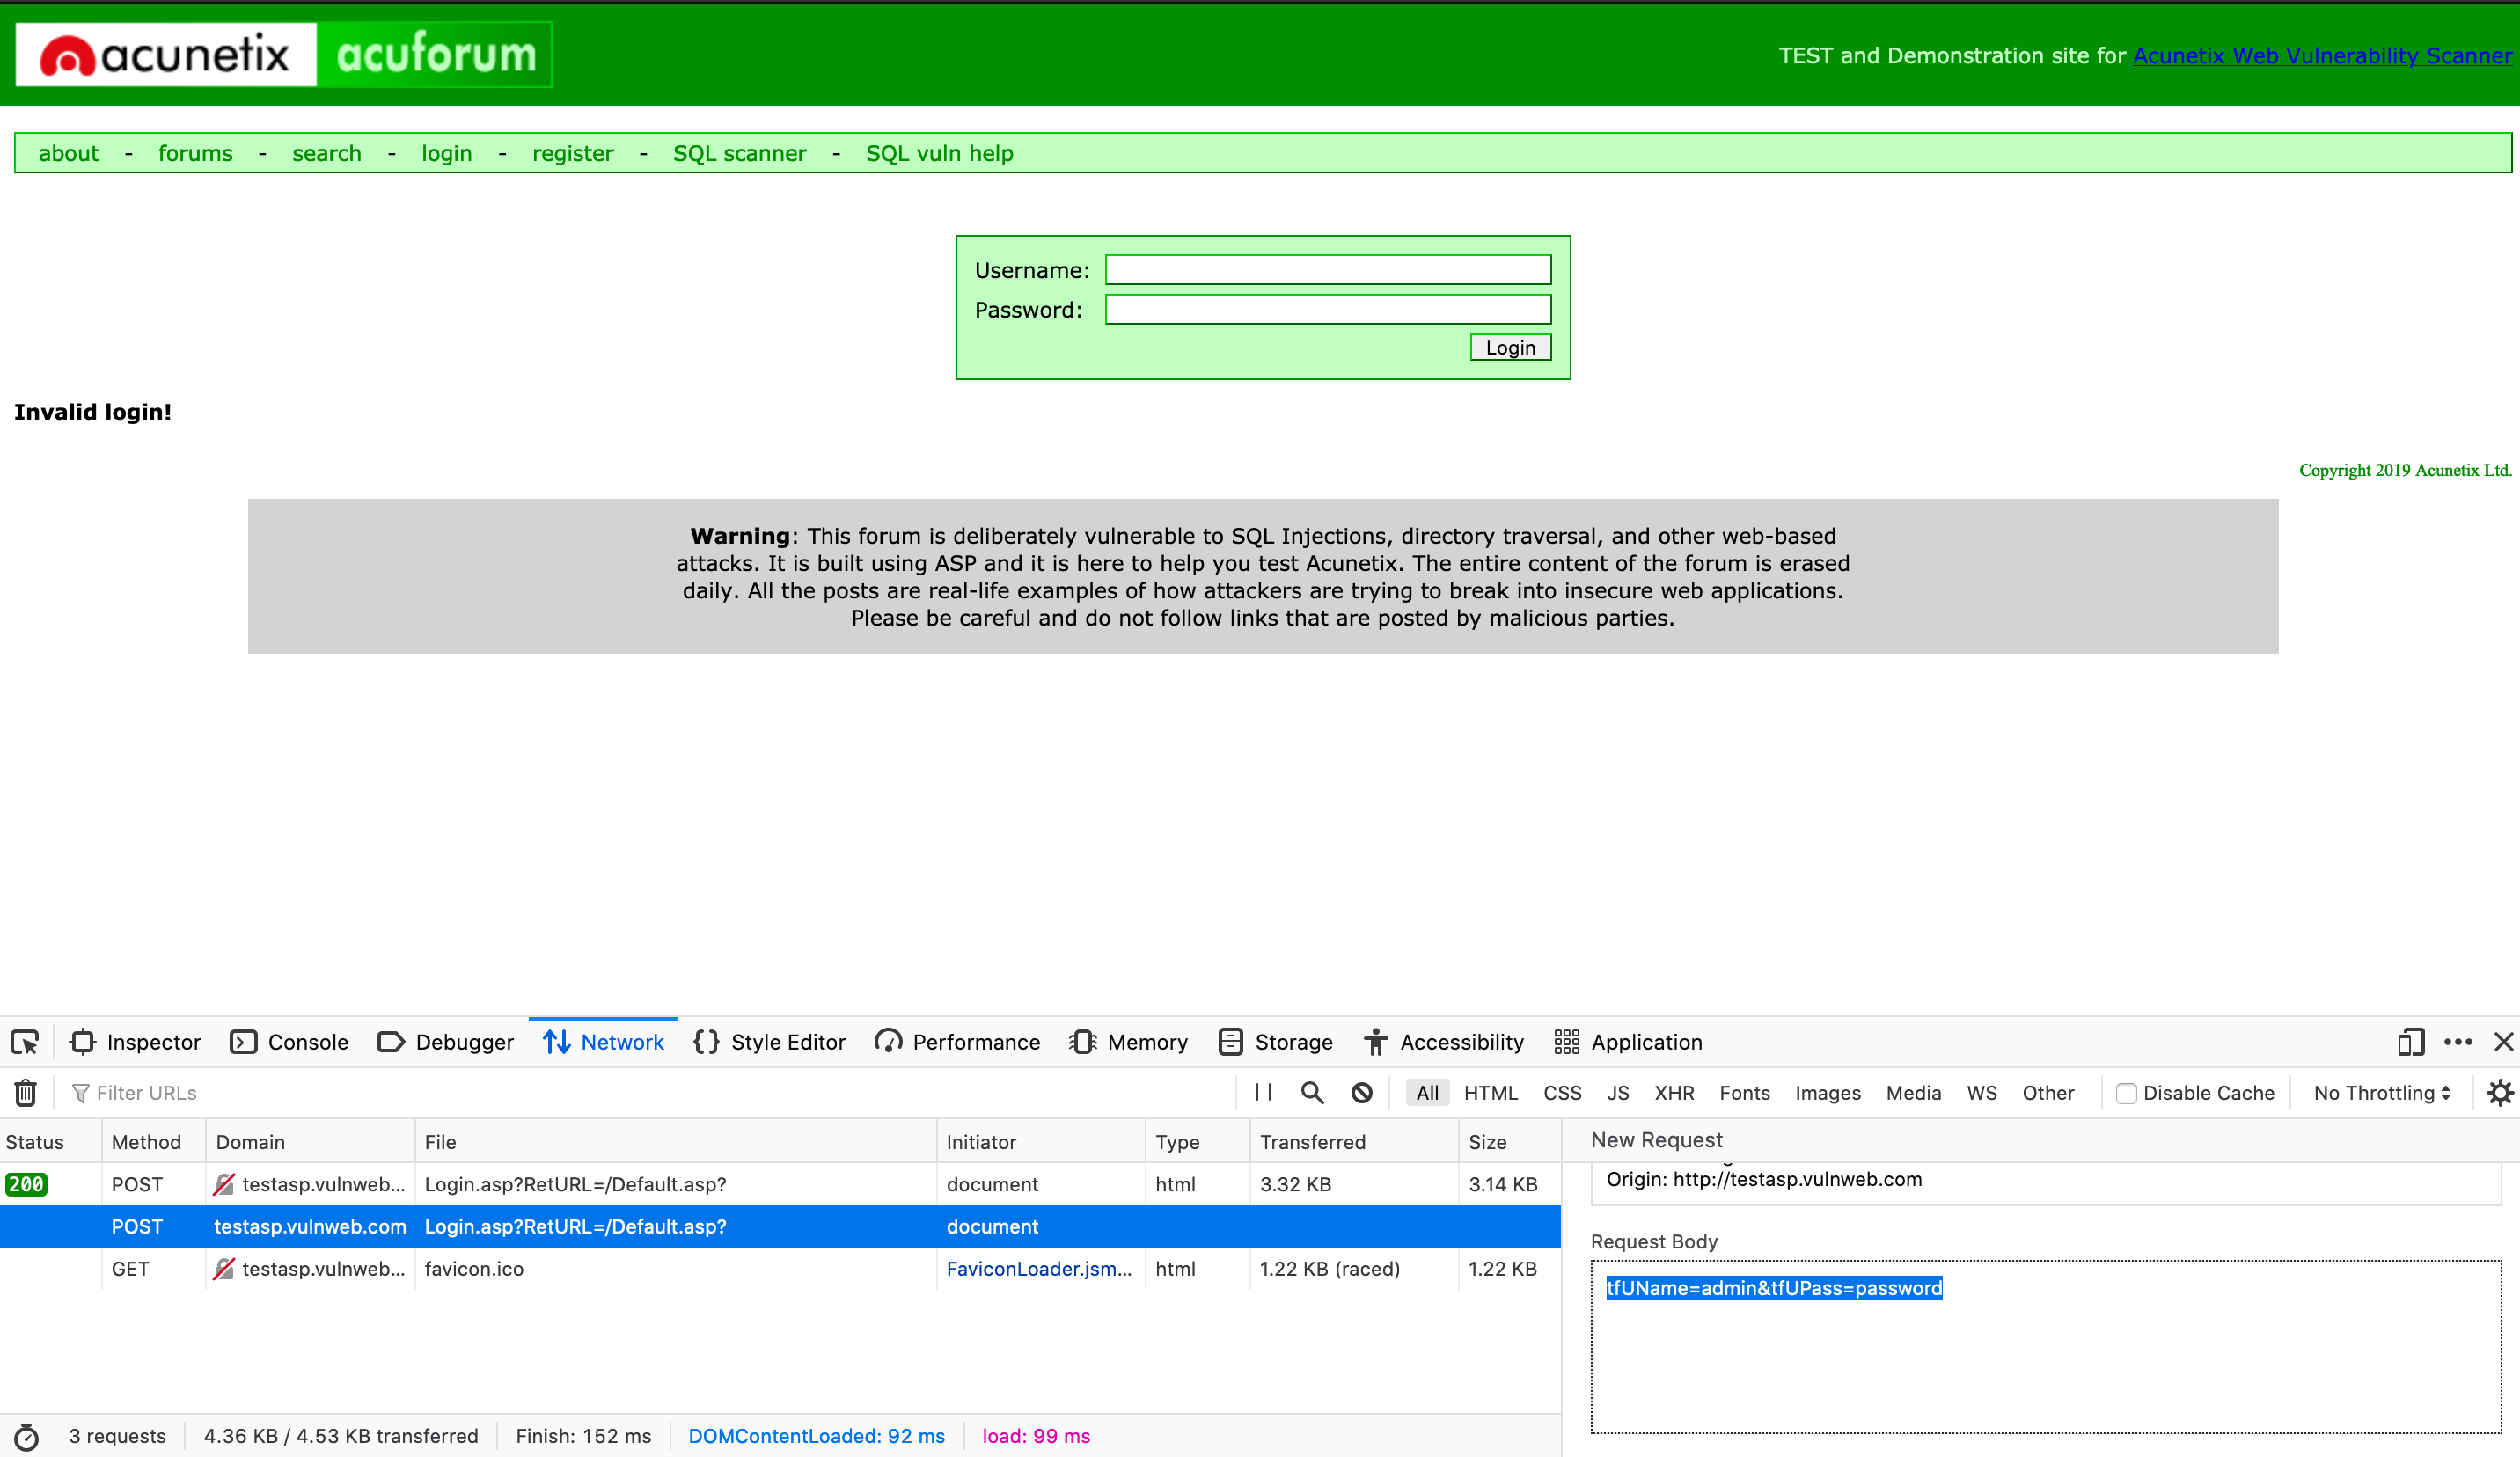
\includegraphics[width=12cm]{request-body}
  \caption{Copying Request Body.}
\end{figure}

\subsection{Wordlists}
Kali Linux has a bunch of wordlists, so you can choose the appropriate one or just use rockyou.txt from \texttt{/usr/share/wordlists/}. So copy the worlist into your home directory and use \textit{gzip} to unzip the archive. Type \texttt{cat rockyou.txt} to see how many passwords the wordlist contains.

\subsection{Run the attack}
Alright, now that we got all arguments, we are ready to fire up hydra. Here is the command pattern:
\begin{lstlisting}
  hydra -l <username> -P <password list> <Target hostname>
  <service module>  <post request parameters>[/code]
\end{lstlisting}
Based on information we have gathered, our command should look something like this:
\begin{lstlisting}
  hydra -l admin -P /usr/share/wordlists/rockyou.txt
  testasp.vulnweb.com http-post-form
  "/Login.asp?RetURL=\%2FDefault\%2Easp\%3F:tfUName=
  ^USER^&tfUPass=^PASS^:S=logout" -vV -f
\end{lstlisting}
Let’s break down the commands:
\begin{itemize}
  \item \textbf{-l <username>:} user name (not hard to guess), use -L <FILE> for a list of possible user names from a file.
  \item \textbf{-P <FILE>:} file with passwords, use -p <password> to literally use one password instead of guessing it.
    testapp.vunlwebapp.com : is a hostname or target
    http-post-form : is the service module we use
    “/Login.asp?RetURL=%2FDefault%2Easp%3F:tfUName=^USER^&tfUPass=^PASS^:S=logout” = the 3 parameters needed, the syntax is :
    {page URL}:{Request post body form parameters}:S={Find whatever in the page after succesfully logged in}
    v = Verbose mode
    V = show login:pass for each attempt
    f = Terminate program if pair login:password is found

\end{document}
